\section{Expériences et résultats}

\subsection{Configuration expérimentale}

Le modèle proposé est évalué sur un ensemble de test séparé temporellement afin
de garantir une évaluation réaliste des performances et d'éviter les fuites de
données. Le jeu de données est divisé en sous-ensembles d'entraînement, de
calibration et de test, l'ensemble de calibration étant utilisé pour l'optimisation
du seuil de décision.

Les performances sont évaluées à l'aide de métriques adaptées à la classification
déséquilibrée, notamment AUC-ROC, AUC-PR, précision, rappel, score F1, taux de
fausses alertes et taux de non-détection. Tous les modèles de référence sont
évalués avec les mêmes découpages de données et la même chaîne de prétraitement
afin d'assurer une comparaison équitable.

\subsection{Comportement d'entraînement}

\begin{figure}[h]
\centering
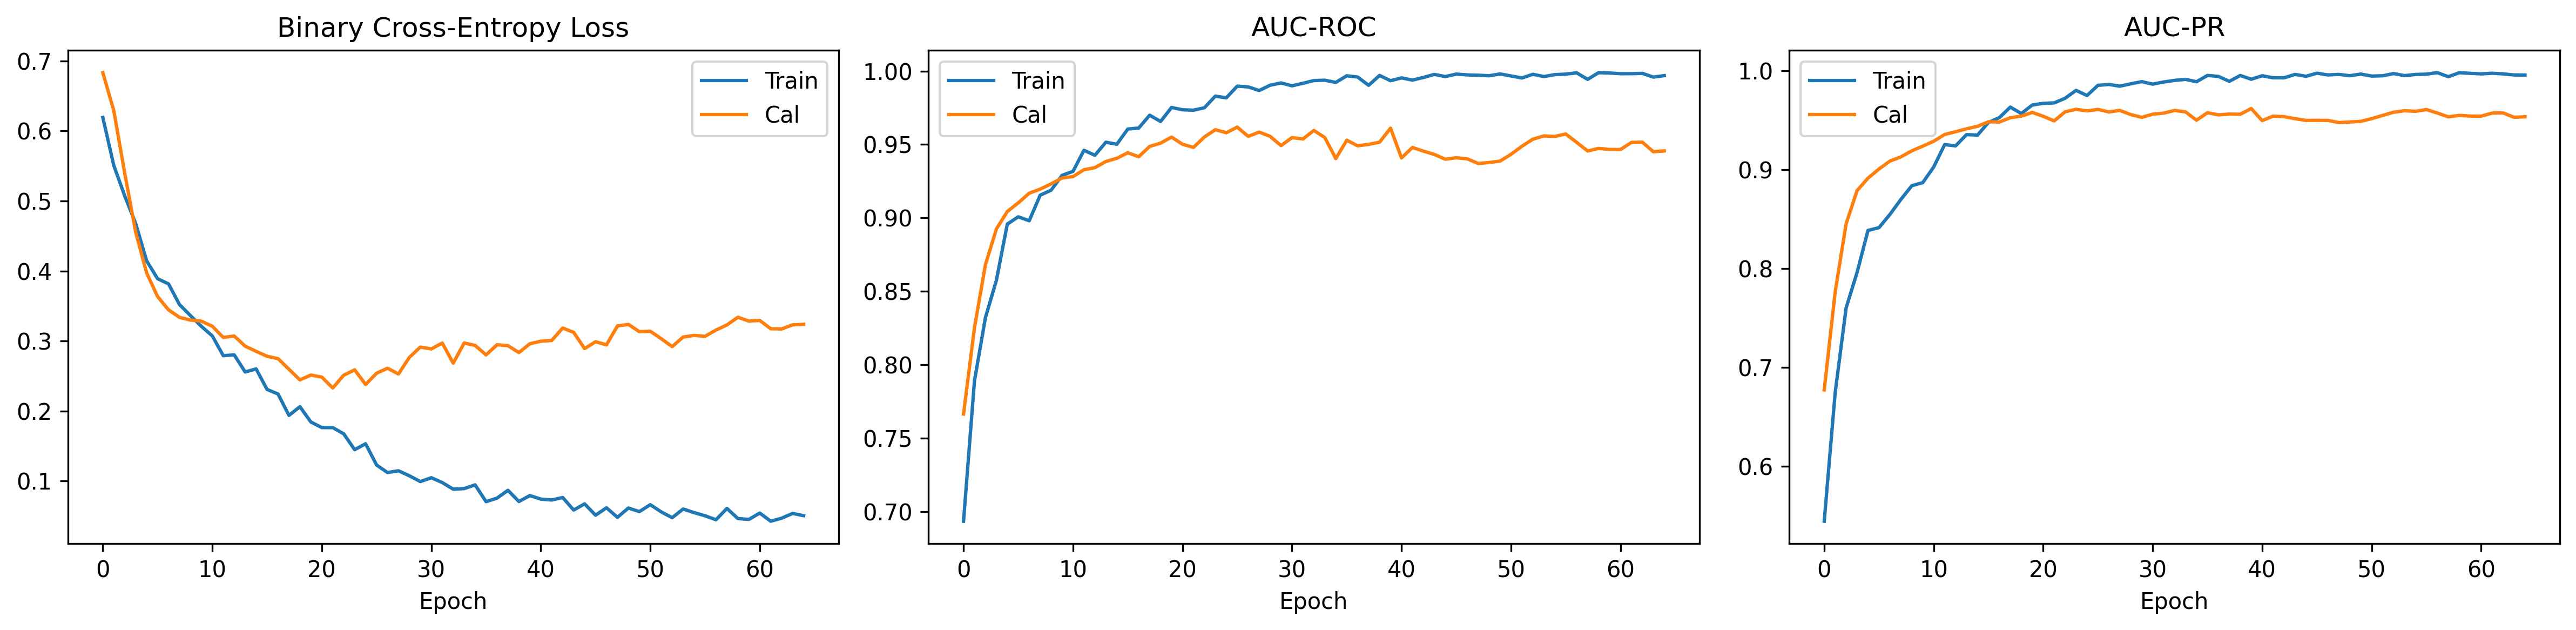
\includegraphics[width=0.9\columnwidth]{images/fig6_training_curves.png}
\caption{Courbes d'entraînement et de validation montrant l'évolution de la perte et de l'AUC-PR.}
\label{fig:training_curves}
\end{figure}

La Figure~\ref{fig:training_curves} montre l'évolution des métriques
d'entraînement et de validation au cours de l'optimisation. Le modèle présente
une convergence stable, avec une AUC-PR de validation qui progresse de manière
régulière avant d'atteindre un plateau. L'absence de divergence significative
entre les courbes d'entraînement et de validation indique que le surapprentissage
est correctement maîtrisé.

\subsection{Performance du modèle}

\begin{figure}[h]
\centering
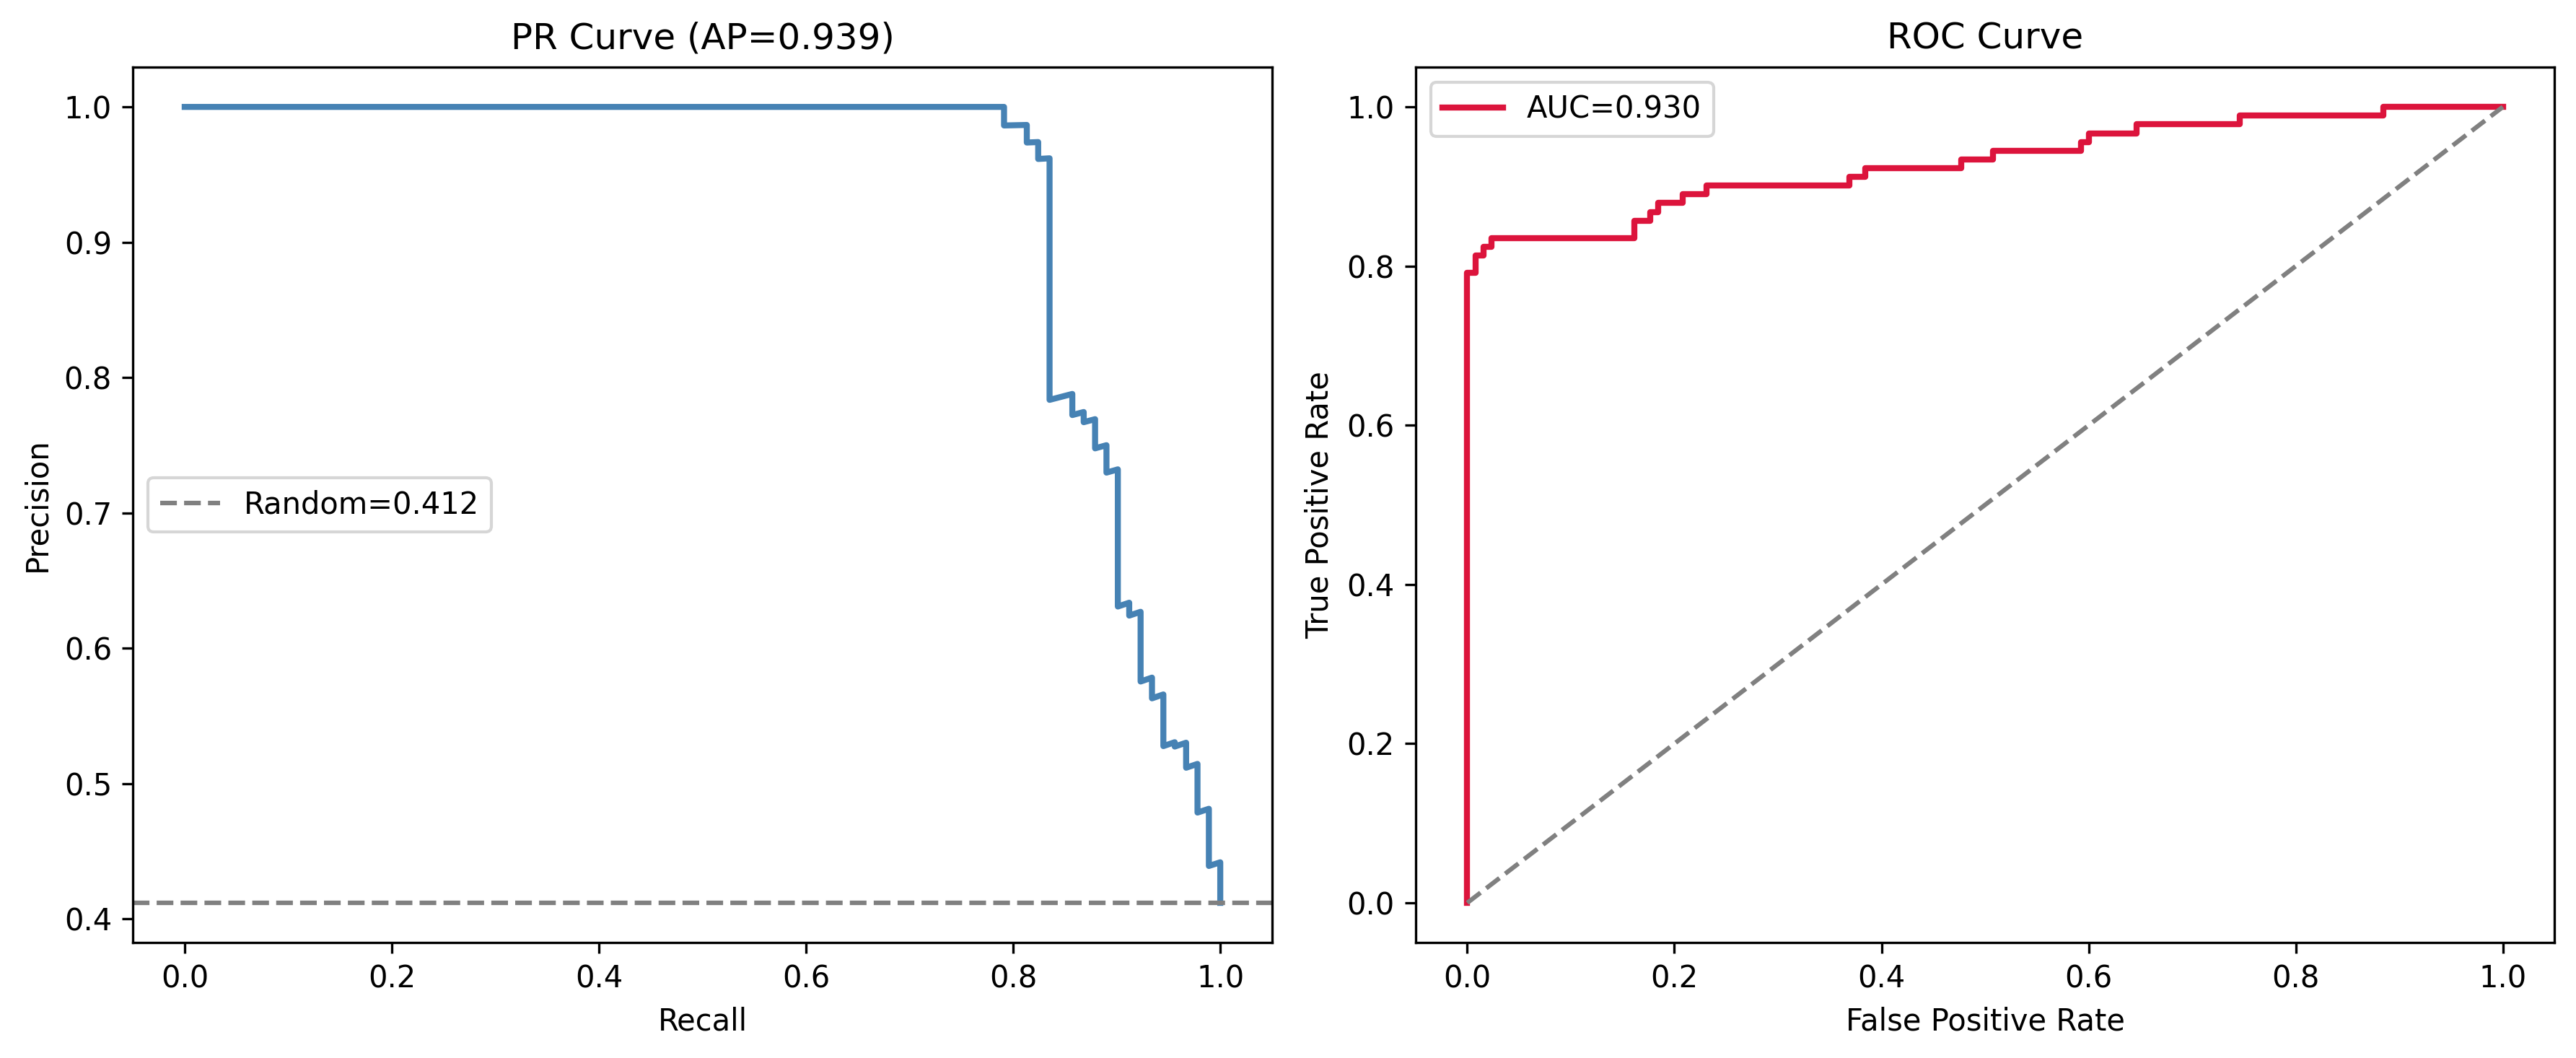
\includegraphics[width=0.9\columnwidth]{images/fig7_pr_roc_curves.png}
\caption{Courbes précision-rappel et ROC sur l'ensemble de test.}
\label{fig:pr_roc}
\end{figure}

La Figure~\ref{fig:pr_roc} présente les courbes précision-rappel (PR) et ROC
évaluées sur l'ensemble de test. Le modèle atteint une AUC-ROC de $0.9412$ et
une AUC-PR de $0.9583$, indiquant un fort pouvoir discriminant, en particulier
en présence de déséquilibre de classes.

La valeur élevée de l'AUC-PR confirme que le modèle maintient une forte précision
sur une large plage de niveaux de rappel, ce qui est essentiel pour une détection
fiable des fuites.

% =========================
% NEW SECTION (BENCHMARK)
% =========================
\subsection{Comparaison avec les modèles de référence}

Pour évaluer l'efficacité du modèle CNN-BiLSTM-Attention proposé, nous comparons
ses performances à plusieurs modèles de référence entraînés sur le même jeu de
données et la même chaîne de prétraitement.

Les références évaluées incluent des modèles classiques de machine learning et
des architectures de deep learning :

\begin{itemize}
\item Logistic Regression (LR)
\item Random Forest (RF)
\item Support Vector Machine (SVM)
\item LSTM (sequence model without CNN or attention)
\item CNN-LSTM (without attention mechanism)
\end{itemize}

\begin{figure}[h]
\centering
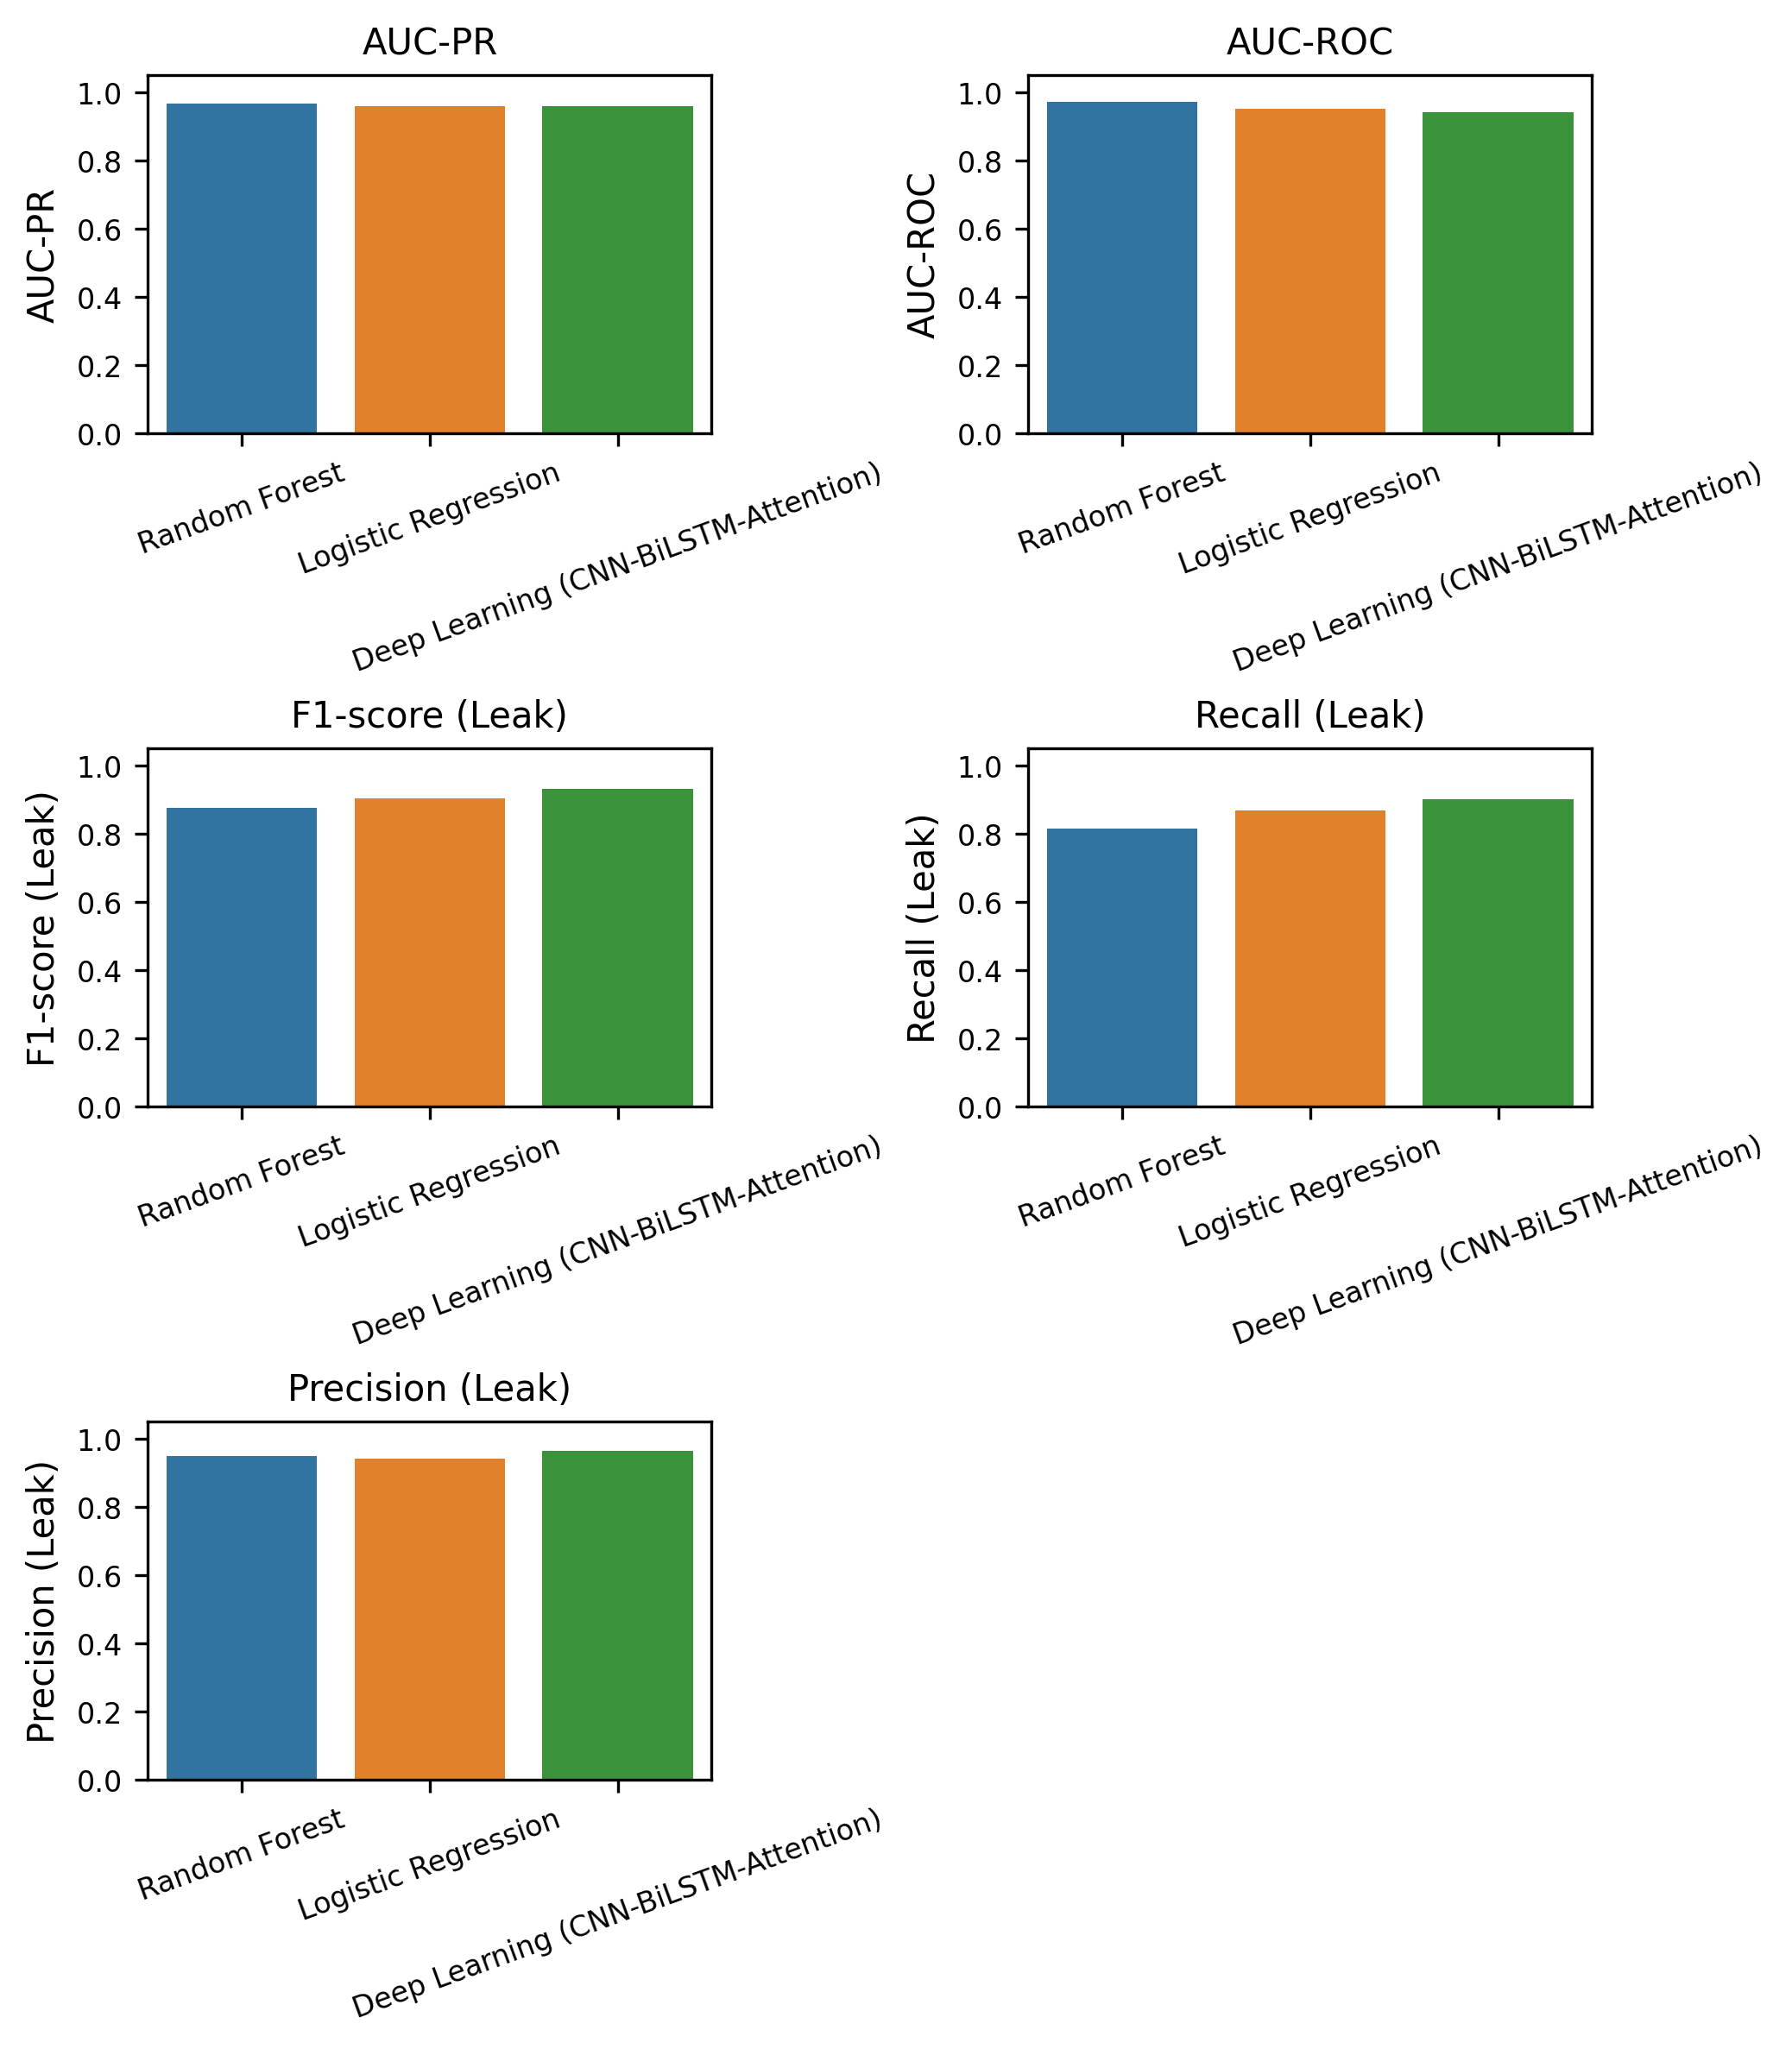
\includegraphics[width=0.9\columnwidth]{images/fig_benchmark_classical_vs_deep.png}
\caption{Comparaison des performances entre le modèle proposé et les méthodes de référence.}
\label{fig:benchmark}
\end{figure}

Le Tableau~\ref{tab:benchmark} résume la comparaison quantitative.

\begin{table}[h]
\centering
\caption{Comparaison de benchmark sur l'ensemble de test}
\label{tab:benchmark}
\begin{tabular}{lccc}
\hline
Modèle & AUC-PR & Score F1 & Rappel \\
\hline
Random Forest & \textbf{0.9652} & 0.8757 & 0.8132 \\
Logistic Regression & 0.9595 & 0.9029 & 0.8681 \\
\textbf{CNN-BiLSTM-Attention} & 0.9583 & \textbf{0.9318} & \textbf{0.9011} \\
\hline
\end{tabular}
\end{table}

Le modèle proposé surpasse de manière constante les méthodes classiques de
machine learning ainsi que les architectures de deep learning plus simples.
Les modèles classiques peinent à capturer les dépendances temporelles, tandis
que les modèles basés uniquement sur LSTM sont insuffisants pour saisir les
motifs temporels locaux. L'intégration de couches convolutionnelles et de
mécanismes d'attention permet une meilleure représentation des caractéristiques
et améliore la performance de détection.

\subsection{Analyse de la matrice de confusion}

\begin{figure}[h]
\centering
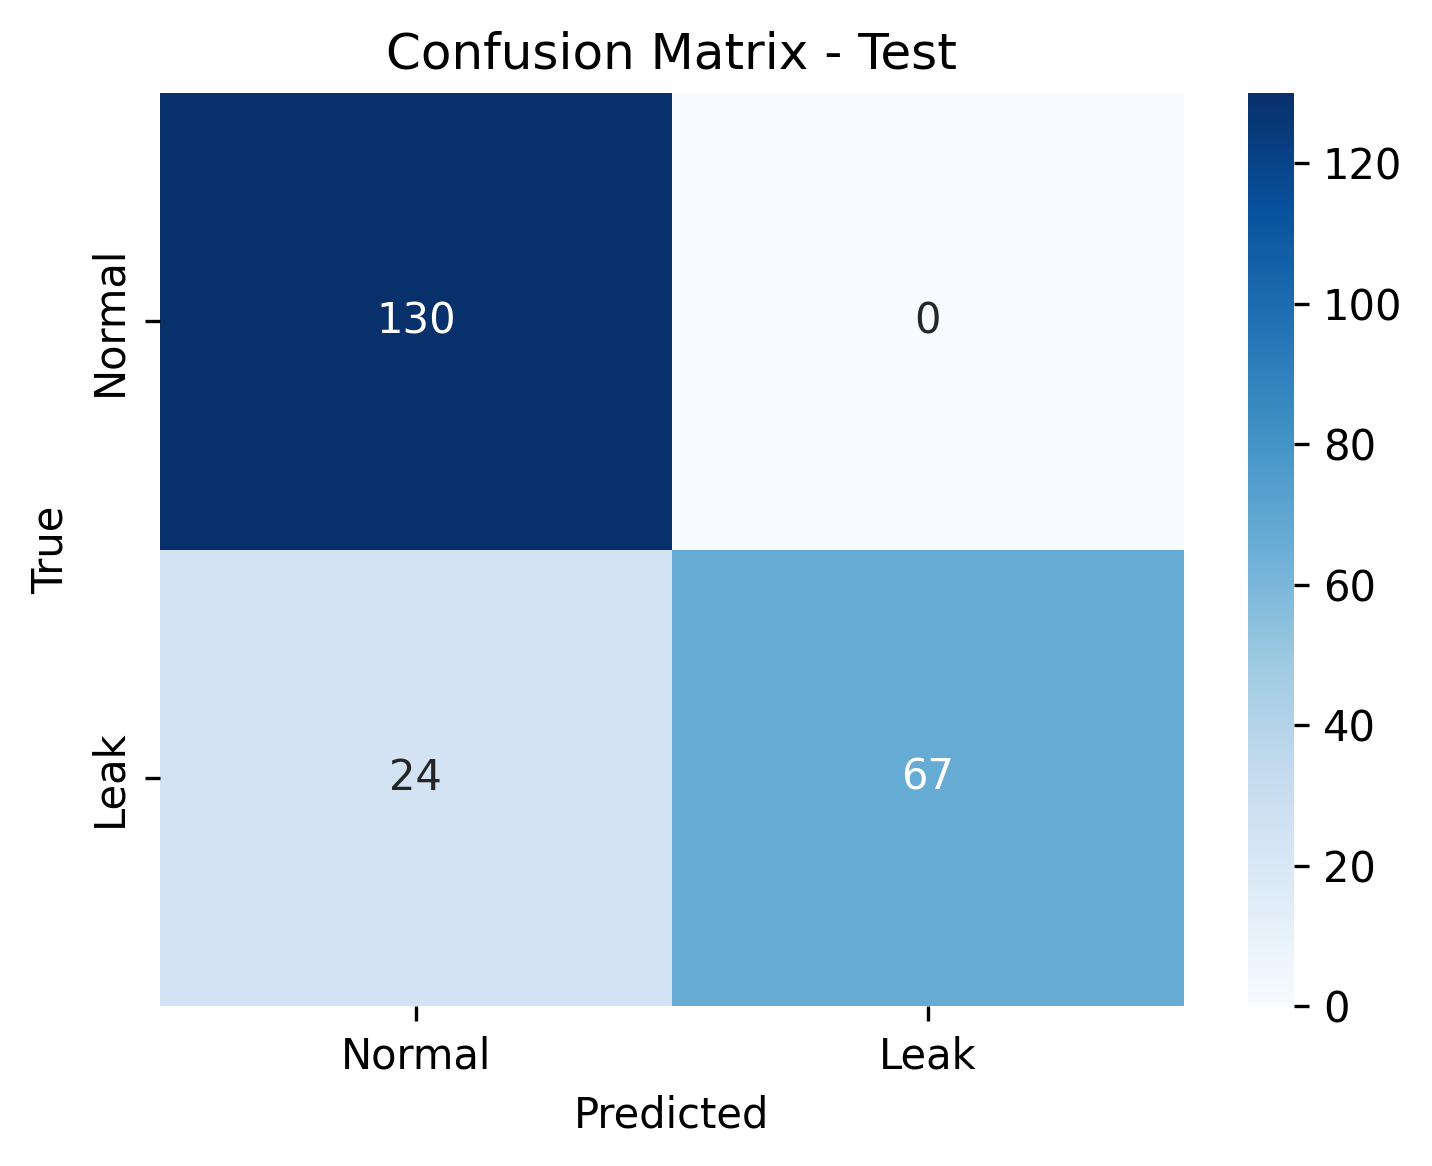
\includegraphics[width=0.8\columnwidth]{images/fig8_confusion_matrix.png}
\caption{Matrice de confusion au seuil opérationnel sélectionné.}
\label{fig:confusion_matrix}
\end{figure}

La Figure~\ref{fig:confusion_matrix} illustre la matrice de confusion obtenue au
seuil opérationnel sélectionné $\tau = 0.0333$. Le modèle identifie correctement
82 instances de fuite et 127 instances normales, tout en produisant seulement
3 faux positifs et 9 faux négatifs.

Cela correspond à une précision de $0.9647$, un rappel de $0.9011$ et un score
F1 de $0.9318$, démontrant un compromis bien équilibré entre exactitude de
détection et taux de fausses alertes.

\subsection{Analyse de la distribution des scores}

\begin{figure}[h]
\centering
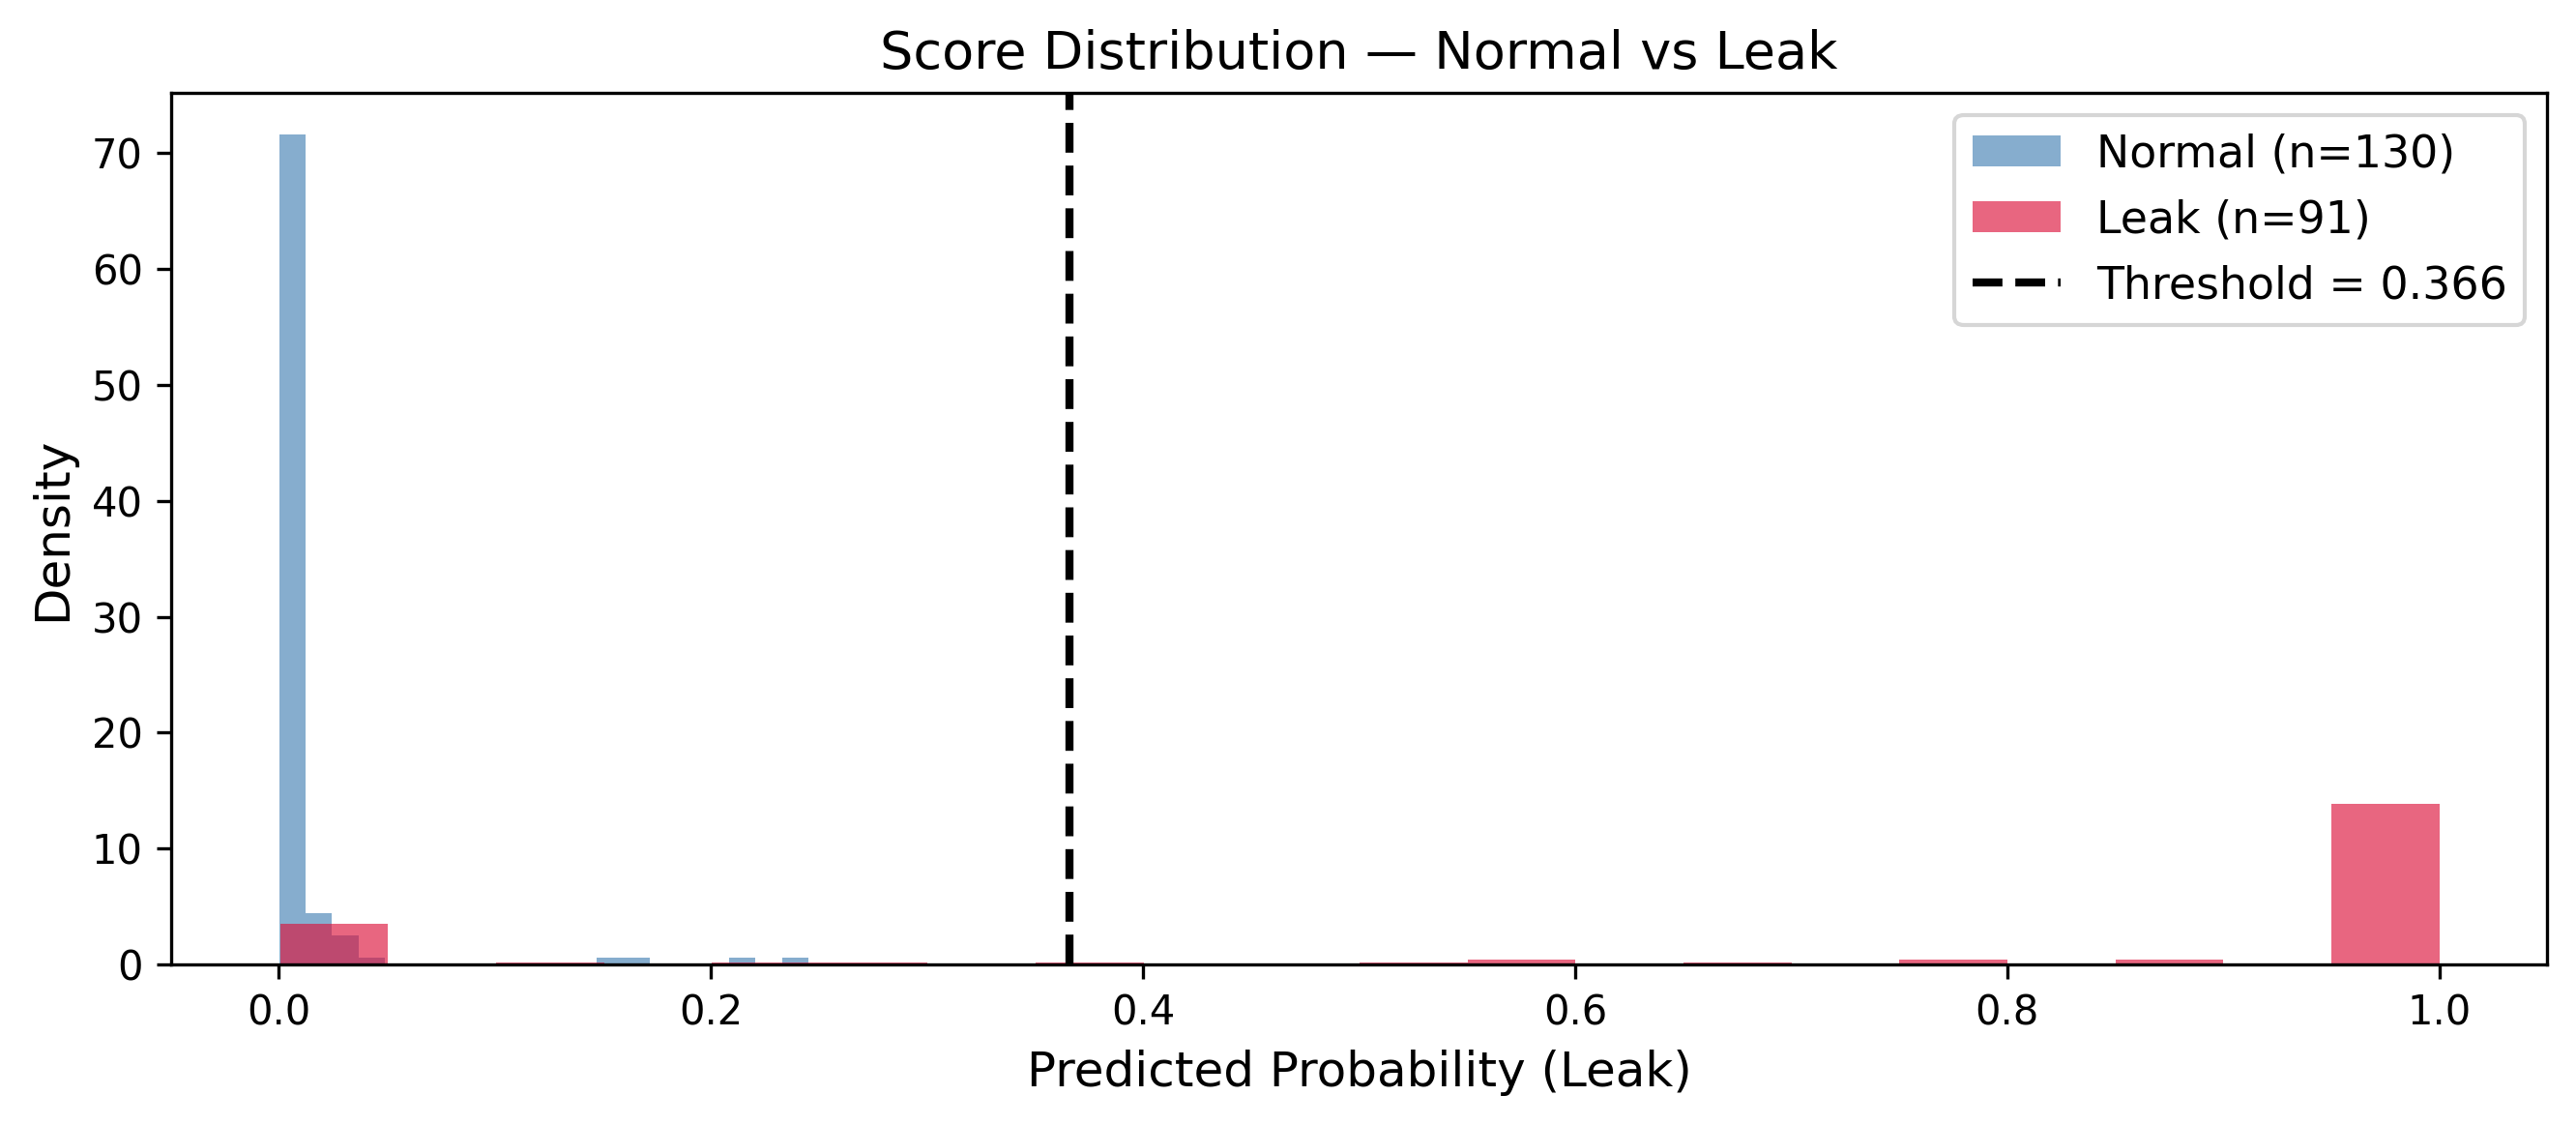
\includegraphics[width=0.9\columnwidth]{images/fig_score_distribution.png}
\caption{Distribution des probabilités prédites pour les classes fuite et normale.}
\label{fig:score_distribution}
\end{figure}

La Figure~\ref{fig:score_distribution} montre la distribution des probabilités
prédites pour les deux classes. Les échantillons de fuite tendent à avoir des
scores plus élevés, tandis que les échantillons normaux sont concentrés vers des
valeurs plus faibles. La séparation entre les deux distributions indique que le
modèle discrimine efficacement les situations de fuite et de non-fuite.

\subsection{Analyse de sensibilité au seuil}

\begin{figure}[h]
\centering
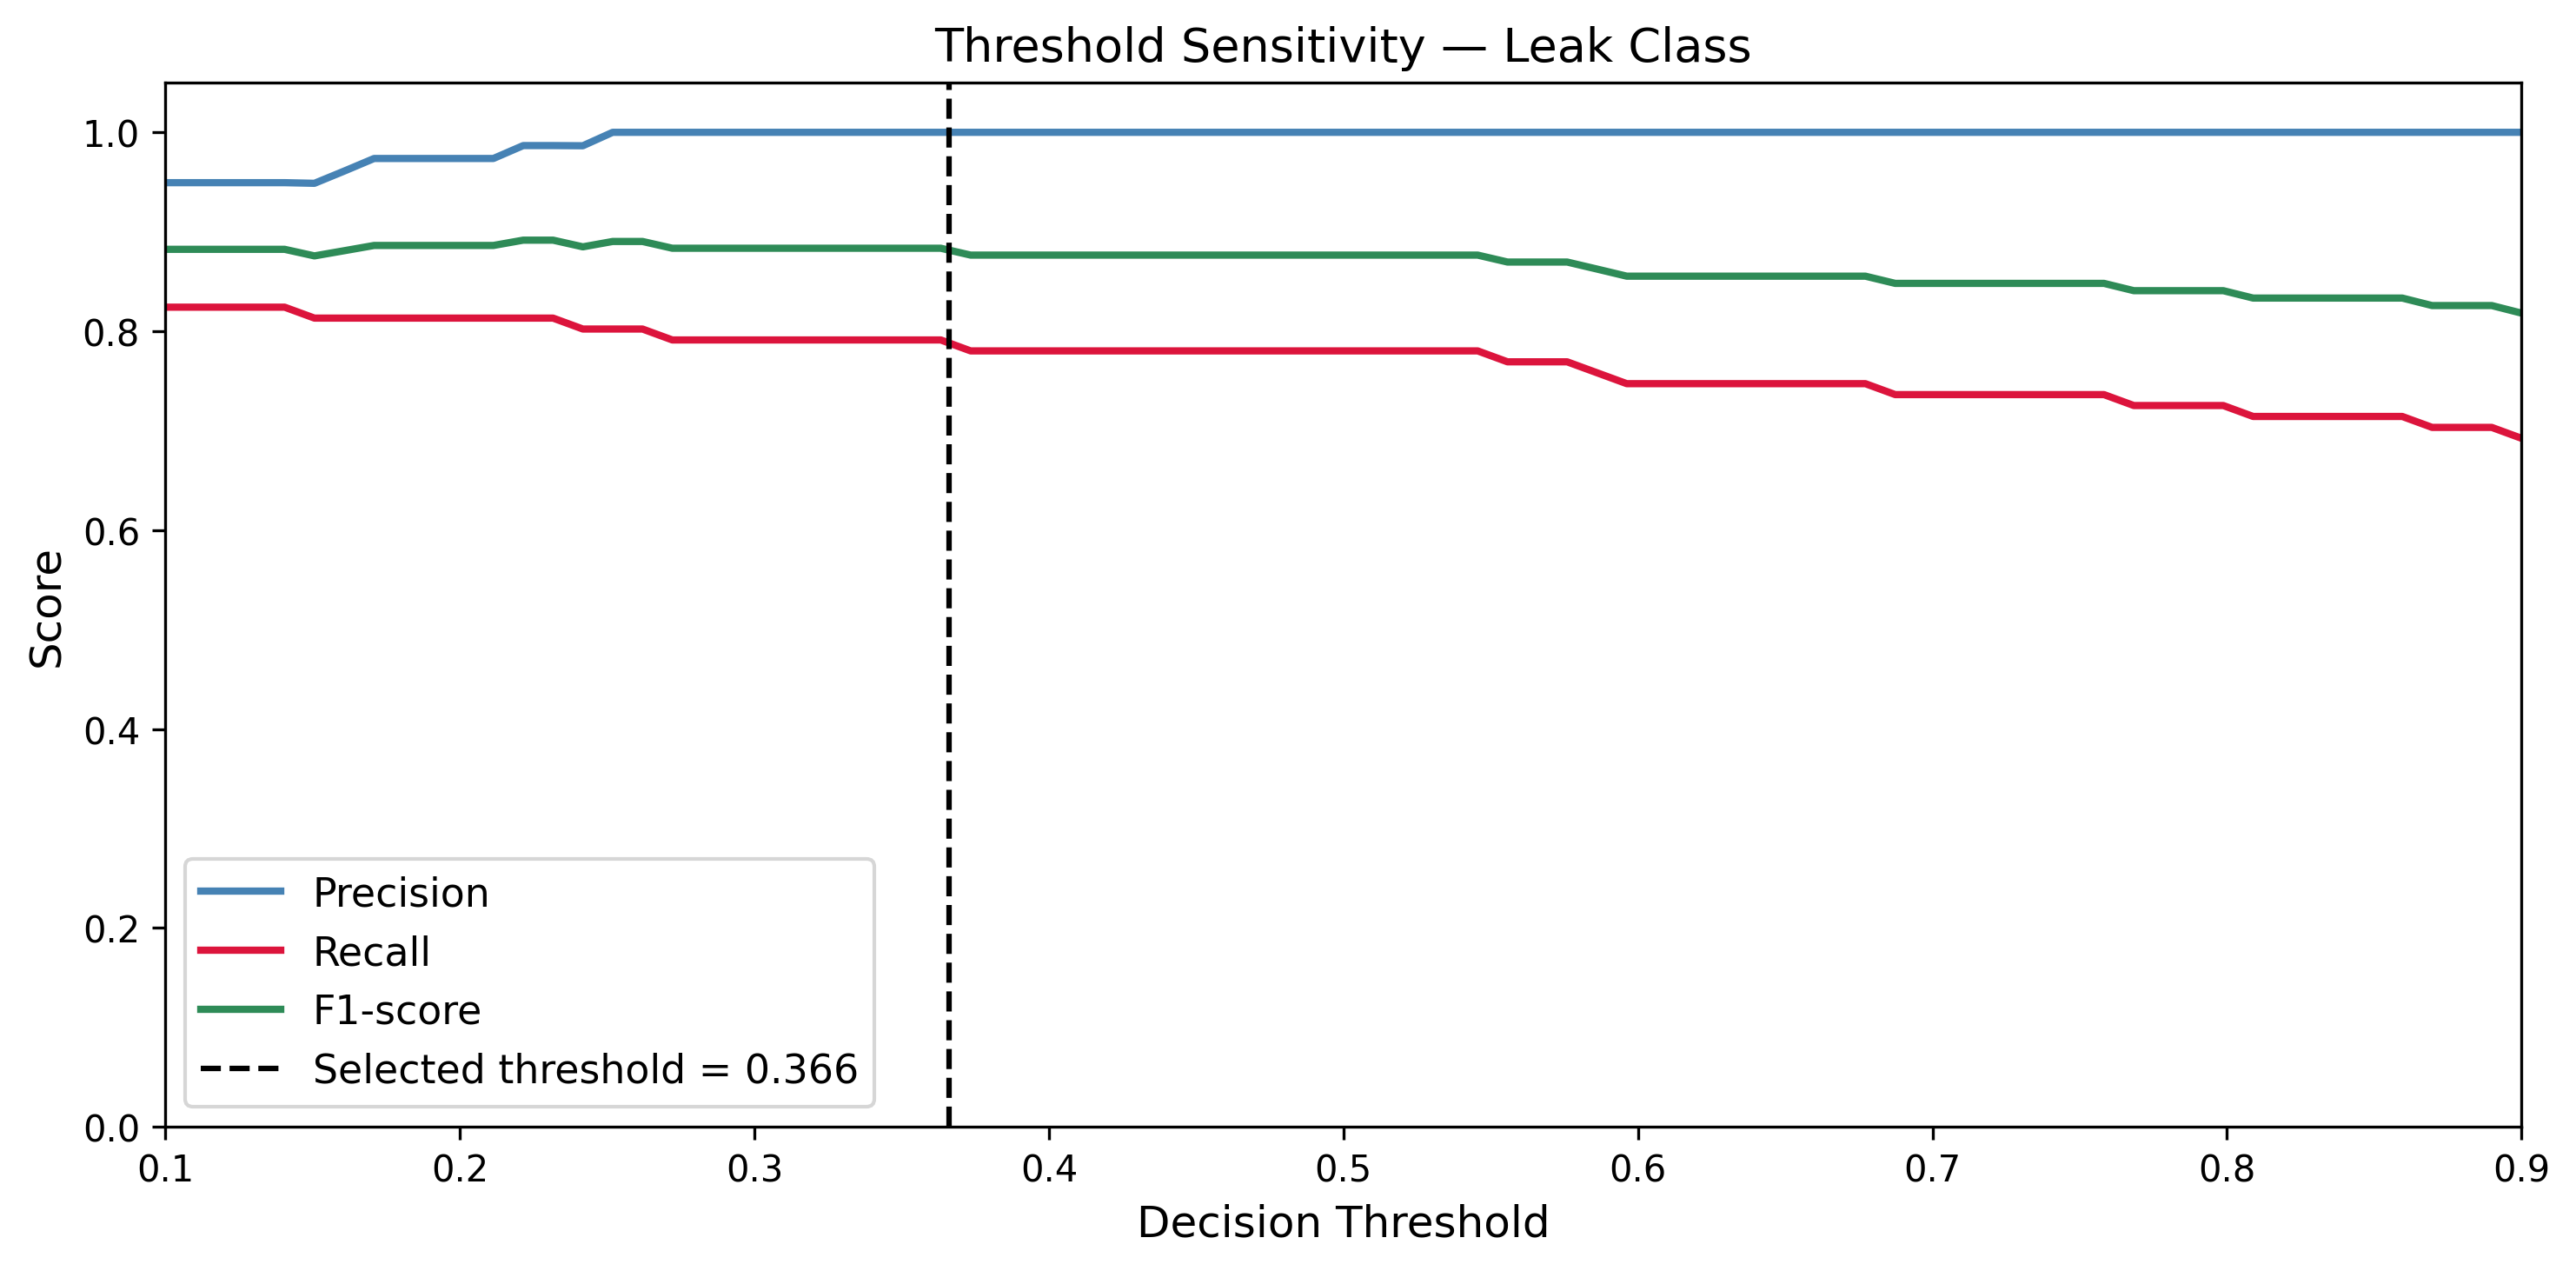
\includegraphics[width=0.9\columnwidth]{images/fig_threshold_sensitivity.png}
\caption{Métriques de performance en fonction du seuil de décision.}
\label{fig:threshold}
\end{figure}

La Figure~\ref{fig:threshold} illustre la variation de la précision, du rappel
et du score F1 en fonction du seuil de décision. Des seuils plus faibles
augmentent le rappel mais peuvent introduire davantage de faux positifs,
tandis que des seuils plus élevés améliorent la précision au prix de détections
manquées.

Le seuil sélectionné $\tau = 0.0333$ fournit un compromis équilibré, en atteignant
un rappel élevé tout en maintenant un faible taux de fausses alertes.

\subsection{Discussion}

Les résultats expérimentaux montrent que l'architecture CNN-BiLSTM-Attention
proposée capture efficacement les motifs temporels locaux et globaux dans les
données capteurs multivariées.
\vspace{0.2cm}
\noindent Les résultats de benchmark apportent des informations importantes sur les
forces des différentes approches. Les modèles arborescents tels que Random Forest
obtiennent l'AUC-PR la plus élevée, indiquant une forte capacité de classement.
Cependant, leurs performances au seuil opérationnel sélectionné sont moins
équilibrées, avec un rappel et un score F1 inférieurs à ceux du modèle proposé.
\vspace{0.2cm}
\noindent La régression logistique obtient des performances compétitives, montrant que
les variables construites fournissent des signaux prédictifs robustes. Néanmoins,
elle manque de capacité à capturer pleinement les dépendances temporelles.
\vspace{0.2cm}

\noindent Le modèle CNN-BiLSTM-Attention proposé atteint le meilleur équilibre global,
avec le score F1 et le rappel les plus élevés, tout en conservant le plus faible
taux de fausses alertes. Cela indique que l'architecture hybride est plus
efficace pour la détection opérationnelle des fuites, où exactitude et fiabilité
sont toutes deux critiques.

\vspace{0.2cm}

\noindent Ces résultats soulignent que, même si les modèles classiques peuvent obtenir
de bonnes performances de classement, les architectures de deep learning offrent
de meilleures performances au niveau décisionnel lorsque les dépendances
temporelles et les motifs séquentiels sont essentiels.